\section{Experimental results}


% \begin{figure}[h!]
% \begin{center}
%  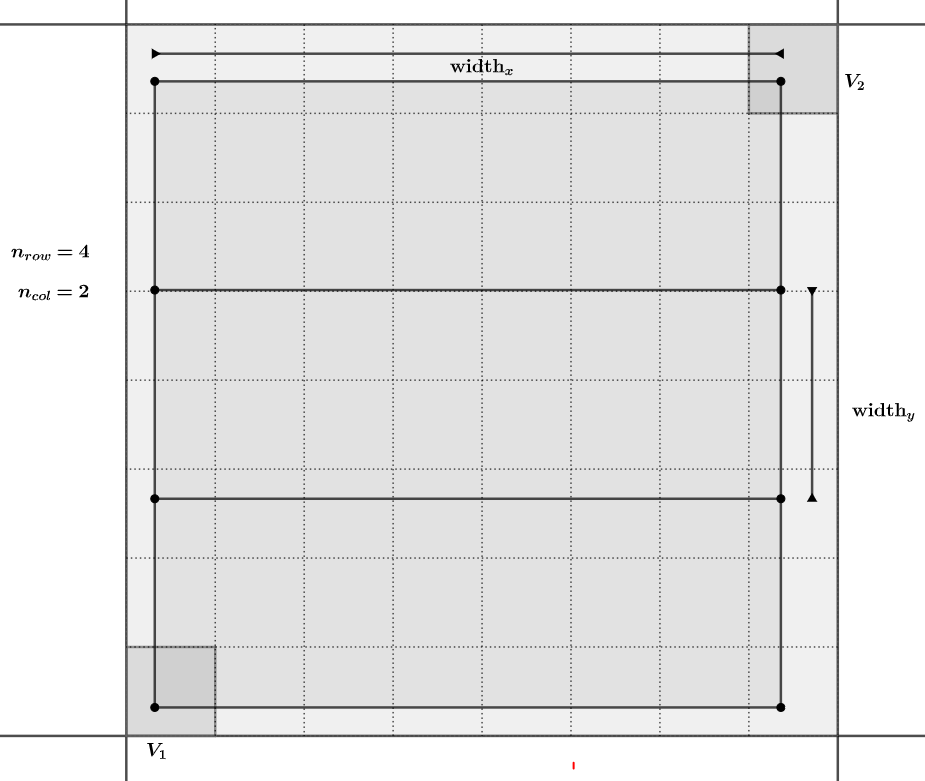
\includegraphics[width=1\linewidth]{Grid_generation.png}
% \end{center}
% \end{figure}
\noindent
In this section we discuss the experimental results obtained testing the formulations presented in Section \ref{Form} and the matheuristic procedure proposed in Section \ref{Math} on different sets of instances. In particular, we generated two sets of instances of the \AMD\xspace problem. The first one consists of targets, to be visited by the drone, that are represented by grid graphs, while the second one involves a different typology of targets, that is, Delaunay graphs. 
For both typologies we generated 5 instances of 10 graphs each, with different cardinality of the set of nodes. More precisely, each instance is composed of 3 graphs with 4 nodes, 3 graphs of 6 nodes, 3 graphs of 8 nodes and 1 graph of 10 nodes. Moreover, we assumed that the drone's speed is twice that of the mothership and that a percentage equal to $80\%$ of each target must be visited by the drone.\\
In order to locate in the space the 10 graphs of a single instance, we considered a square of side 100 units. Then we divided the original square in subsquares of side 5 and we randomly selected among them the locations for the ten target graphs of the instance. The generation procedure of the single graph in a selected square, depends on the graph typology.
As regards grid graphs, the single subsquare, like the one represented in Figure \ref{fig:fig1}, is further partitioned in subsquares of side $\frac{5}{n}$ where $n$ is the cardinality of the set of nodes of the graph to build. Two opposite corner subsquares have been considered (like $V_1$ and $V_2$ in Figure \ref{fig:fig1}) and one point inside each of them was randomly selected (black points in the subsquares $V_1$ and $V_2$ in Figure \ref{fig:fig1}). Then, a rectangle whose diagonal joins these two points has been built (the black dotted one in Figure \ref{fig:fig1}). A grid of $n$ points has been identified by locating $\frac{n}{m}$ 
%\CV{here we have n/m rows and m columns selected randomly in the set of divisors of the number of points of the graph)}
equally spaced points on the two sides square (the red ones and the two original points in black in Figure \ref{fig:fig1}), where $m$ is randomly selected in the set of divisors of the number of points of the graph. The links of the graphs connect each point to its adjacent ones lying on the same side and with the one located on the opposite side of the square.  Let $width_x$ and $width_y$ be the lengths  of these edges as show in Figure \ref{fig:fig1}. In order to perturb the coordinates of these points, we randomly added a value, ranging between $-\frac{width_x}{3}$ and $\frac{width_x}{3}$ to the $x$ coordinate and between $-\frac{width_y}{3}$ and $\frac{width_y}{3}$ to the $y$ coordinate, always imposing that the perturbed point still belongs to the square. The resulting grid graph is obtained connecting the same pairs of points but with perturbed coordinates (blue graph in Figure \ref{fig:fig1}). \\
As regards the instances related to Delaunay graphs, we adopted the same procedure as for the grid ones, for selecting their locations in the space. Then, for each randomly selected subsquare, given the set of $n$ nodes of the graph to be generated, a Delaunay triangulation of them is computed by using the Python class scipy.spatial.Delaunay (see \cite{art:Virtanen2020} for further details).





\begin{figure}[h!]
\begin{center}
 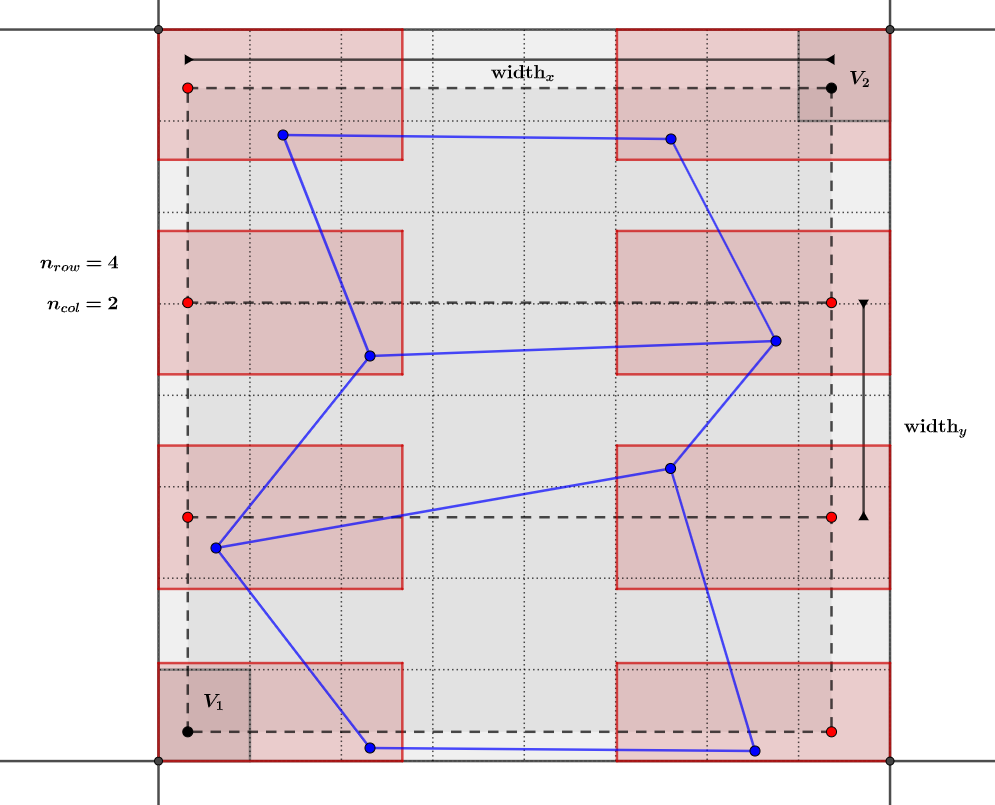
\includegraphics[width=0.6\linewidth]{Grid_generation_2.png}
\end{center}
\caption{Example of generation of a grid graph}
\label{fig:fig1}
\end{figure}
 
 
\noindent
We run the three formulations proposed in Section \ref{Form} for the \AMD\xspace problem (Stages, MTZ and SEC) with two different commercial solvers, Cplex 12.8 and Gurobi 9.03, called by means of Python, by setting a time limit for each run equal to 3600 sec.
In Table \ref{table:tab1} we reported the results obtained, in terms of average, minimum and maximum percentage with both solvers, on the instances consisting of grid graphs. First, we can observe that Gurobi has better performances with respect to Cplex for all the instances. Moreover, for this set of instances, the SEC formulation is the best one among the three proposed, as the associated average gap is equal to 0.61\% and also the minimum and the maximum percentage gap are smaller than the ones associated with the Stages and the MTZ formulations.\\

 
\renewcommand{\arraystretch}{0.7}
\begin{table}[!h]
\caption{Comparison between formulations for grid instances}
\centering
\footnotesize
\begin{tabular}{c | c c | c c | c c}
\hline\hline
\textbf{Gap \%} & \multicolumn{2}{c}{Average} &  \multicolumn{2}{c}{Min} &  \multicolumn{2}{c}{Max} \\
 % \hline
\textbf{Solver} &Cplex &Gurobi &Cplex &Gurobi  &Cplex &Gurobi \\
\hline
\textbf{Formulation} & & & & & &\\
Stages & 0,87 &	0,87 &	0,85 &	0,84 &	0,88 &	0,88\\
MTZ	 & 0,66 &	0,62 &	0,59 &	0,58 &	0,72 &	0,65\\
SEC	& 0,65 &	0,61 &	0,59 &	0,57 &	0,70 &	0,64\\
    \hline
\end{tabular}
\label{table:tab1}
\end{table}


\noindent
Similarly, Table \ref{table:tab2} summarizes the results obtained on the instances with Delaunay graphs. Also in this case the Gurobi performances are better than Cplex. However, among the three formulations, the MTZ one provides the best results in terms of average and maximum percentage gap.



\renewcommand{\arraystretch}{0.7}
\begin{table}[!h]
\caption{Comparison between formulations for Delauney instances}
\centering
\footnotesize
\begin{tabular}{c | c c | c c | c c}
\hline\hline
\textbf{Gap \%} & \multicolumn{2}{c}{Average} &  \multicolumn{2}{c}{Min} &  \multicolumn{2}{c}{Max} \\
 % \hline
\textbf{Solver} &Cplex &Gurobi &Cplex &Gurobi  &Cplex &Gurobi \\
\hline
\textbf{Formulation} & & & & & &\\
Stages &	0,91 &	0,91 &	0,90 &	0,89 &	0,93 &	0,93\\
MTZ	& 0,78 &	0,74 &	0,74 &	0,70 &	0,82 &	0,79\\
SEC	& 0,77 &	0,75 &	0,73 &	0,69 &	0,82 &	0,81\\
    \hline
\end{tabular}
\label{table:tab2}
\end{table}


\noindent
In order to test the performances of the matheuristic proposed in Section \ref{Math}, we coded it in Python and we run it on the same sets of instances (Grid and Delaunay) on which the three formulations have been solved. Table \ref{table:tab3} reports for each instance, numbered from 0 to 4, distinguishing between Grid and Delauney, respectively, the best objective function provided by the best formulation, the objective function provided by the matheuristic and the associated CPU time. As already noticed from Table \ref{table:tab2}, for grid graph instances, SEC formulation has the best behaviour, with the exception of the instance number 3 for which the MTZ provides a smaller value of the objective function. As for the Delaunay graph instances, MTZ is the best formulation, but also in this case there is an exception on the instance number 2 for which SEC formulation returns a smaller value of the objective function.\\
The results show that the matheuristic returns a solution with value of the objective function that is higher than the one provided by the SEC formulation on grid instances. However, these values are smaller than the ones provided by the Stages and the MTZ formulations. Moreover, the saving in terms of resolution time is very significant as the maximum CPU time is less than 1 minute.  As regards the Delaunay instances, the matheuristic performances are even better, as it finds a solution that is better than the best one provided by the MTZ formulation and in a resolution time that is at most 28 minutes. 



\renewcommand{\arraystretch}{0.7}
\begin{table}[!h]
\caption{Heuristic performances}
\centering
\footnotesize
\begin{tabular}{c | c c c | c c c}
\hline
\textbf{\#}  & \multicolumn{3}{c}{\textbf{Grid}} &  \multicolumn{3}{c}{\textbf{Delauney}} \\
 % \hline
 &Best Obj & Obj Heuristic &CPU Time &Best Obj & Obj Heuristic & CPU Time \\
\hline
0 &	1087,87	& 1117,83 &	50,99 &	947,01 &	934,46 &	52,49\\
1 &	1100,38	& 1319,64 &	24,64 &	986,22 &	 938,68	& 72,73\\
2 &	1350,67	& 1126,35 &	46,06 &	888,48 &	865,66 &	1073,80\\
3 &	1218,66	& 1476,36 &	27,18 &	1249,69 &	1154,62 &	1703,33\\
4 &	1297,77	& 1424,37 &	40,91 &	1239,93	 & 1184,67 &	81,15\\
    \hline
\end{tabular}
\label{table:tab3}
\end{table}


\noindent
We performed a second set of experiments by observing that, even if there are small differences between the SEC and the MTZ formulations depending on the type of instances, their performances are comparable.
Thus, in the rest of the tests we focused on the MTZ formulation. We compared its performances, with or without providing the initial solution found by the matheuristic, on a set of larger instances. More precisely, we generated 20 instances with targets represented by grid graphs and 20 instances with targets represented by Delauney graphs. The instances of each typology are split in 4 groups of 5 instances each, consisting respectively of 5, 10, 15 and 20 targets to be visited.
In each instance the same percentage of graphs ($20\%$) has respectively 4, 6, 8, 10 and 12 nodes. 
Moreover, we assumed that the origin coincides with the destination in all instances and we randomly generated with uniform distribution between 0 and 1, two values representing the percentage of each edge and of each graph to be visited.
As regards the speeds, we set the speed of the drone three times the one of the mothership.
We run the MTZ formulation by adopting Gurobi, setting a time limit of 7200 sec. for each instance.
On the same instances also the matheuristic has been applied. Note that, in order to define a stopping rule for the exact resolution of the \AMD\xspace model within the matheuristic procedure (STEP 3 and STEP 4), we set the maximum number of solutions generated by the solver equal to five.
For each instance, the solution provided by the matheuristic has been then used to initialize the exact resolution of the MTZ formulation in order to try to speed up the resolution process.
Table \ref{table:tab4} shows the results of the comparison between the exact resolution of the formulation with and without initialization. In the first column, named List, we report the size of the instances in terms of number of targets to be visited (0, 1, 2 and 3 identifies instances respectively with 5, 10, 15 and 20 graphs).The second column refers to the two variants of the model, that is, a given percentage of each edge of the targets (e) or a given percentage of each target (g) must be visited by the drone. The other columns report respectively the average percentage gap of the solutions found within the time limit starting from the initial solution provided by the matheuristic, the average running time of the matheuristic and the average percentage gap of the solutions found within the time limit without initialization. These information are reported for both Grid and Delauney instances.

\renewcommand{\arraystretch}{0.7}
\begin{table}[!h]
\caption{Comparison between exact resolution with and without initialization}
\centering
\footnotesize
\begin{tabular}{c c | c c c | c c c}
\hline
 &  & \multicolumn{3}{c}{\textbf{Grid}} &  \multicolumn{3}{c}{\textbf{Delauney}} \\
\hline
 List &  $\%$  & $\%$ Gap (i) & Time$\_$h & $\%$ Gap (ni)  & $\%$ Gap (i) & Time$\_$h &  $\%$ Gap (ni)\\
\hline
\multirow{}{}{0} & e & 0.72 & 105.12 & 0.73 & 0.78 & 154.92 & 0.74\\
& g & 0.55 & 58.92 & 0.54 & 0.62 & 92.64 & 0.67\\
\hline
\multirow{}{}{1} & e & 0.76 & 241.99 & 0.76 & 0.80 & 314.69 & 0.79\\
& g & 0.71 & 182.61 & 0.70 & 0.74 & 353.04 & 0.75\\
\hline
\multirow{}{}{2} & e & 0.76 & 367.69 & 0.76 & 0.80 & 447.61 & 0.80 \\
& g & 0.71 & 326.49 & 0.72 & 0.76 & 429.16 & 0.76\\
\hline
\multirow{}{}{3} & e & 0.75 & 481.68 & 0.74 & 0.80 & 514.98 & 0.76^*\\
& g & 0.71 & 492.27 & 0.70 & 0.77 & 582.90 & 0.77\\
    \hline
\end{tabular}
\label{table:tab4}
\end{table}

\noindent
From Table \ref{table:tab4} we can notice that in most of the cases the average gaps associated with the solution found within the time limit, with and without initialization by the solution found by the matheuristic, are the same or very close (note that in the last column the $*$ indicates that only one instance has been solved within the time limit).
As regards the running time of the matheuristic, we can see also from the boxplots in Figure \ref{fig:1}, that it increases with the number of targets to be visited both for Grid and Delaunay instances. Considering the model variants based on the minimum percentage of each edge or each graph to visit, we can observe that for Grid instances the average running time of the model imposing a minimum percentage of each edge to be visited, is greater than the one associated with the other variant, with the exception of the instances of biggest size (List=3). \\
\noindent
The boxplots in Figure \ref{fig:2} represent the percentage gap of the solution provided by the matheuristic with respect to the one provided by the exact resolution of the MTZ model within the time limit, with initialization by the solution found by the matheuristic. From them we can notice that the gap increases with the size both for Grid and Delaunay instances but it is always less than 0.5$\%$.  
Figure \ref{fig:3} shows the percentage gap of the solution provided by the exact resolution of the MTZ formulation within the time limit without the initialization, with respect to the one found with the initialization. This gap is very close to 0 both for Grid and Delaunay instances. Only for the biggest size we observe values ranging between 0.1$\%$ and 0.6$\%$. These observations suggest that, even if the initialization of the model by the solution provided by the matheuristic does not speed up the convergence to the optimal solution, the matheuristic provides solutions of very good quality. Indeed, it generates in less than 10 minutes solutions that are very close to the ones provided by the model within 2 hours.\\


\begin{figure}[htp]% [H] is so declass\'e!
\centering
\begin{minipage}{0.45\textwidth}
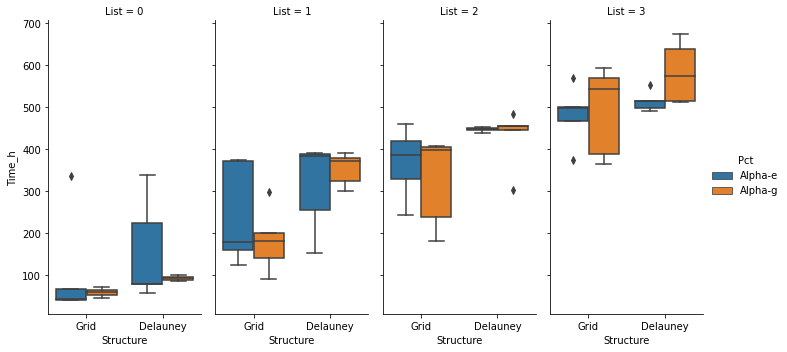
\includegraphics[width=\textwidth]{time_h.png}
\caption{Matheuristic running time}
\label{fig:1}
\end{minipage}\hfill
\begin{minipage}{0.45\textwidth}
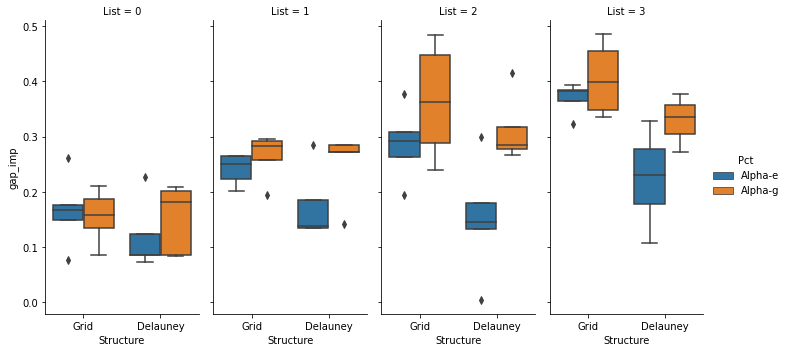
\includegraphics[width=\textwidth]{improved_gap.png}
\caption{Matheuristic improved gap}
\label{fig:2}
\end{minipage}\par
\vskip\floatsep% normal separation between figures
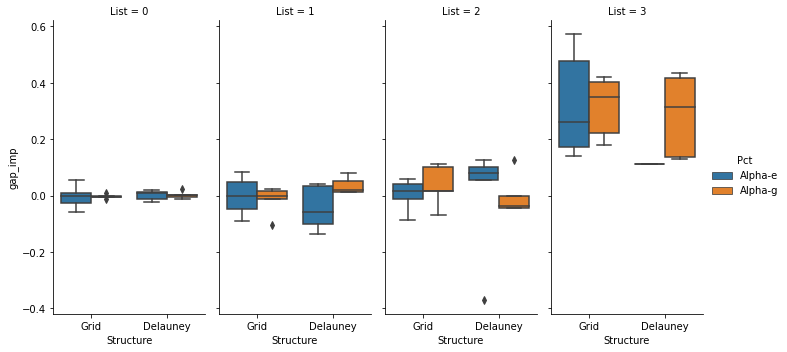
\includegraphics[width=0.45\textwidth]{differencewithwithout.png}
\caption{Improved gap of MTZ formulation with and without initialization}
\label{fig:3}
\end{figure}



\noindent
As regards the \NMD \xspace problem, we generated three sets of instances with targets represented by grid graphs considering different structures of the polygonal network where the mothership can move.
In particular, we defined a first set of instances where the mothership network is represented by a graph of 6 nodes with a tree structure with origin of the path of the base vehicle different from the destination.
A second set of instances involving a mothership network consisting in a complete graph of 4 vertices with origin of the path of the base vehicle different from the destination.  
A third set of instances characterized by star graphs of 7 nodes representing the mothership network, where the origin coincides with the destination and it is located at the centre of the star. We generated 10 instances for each of these three classes, 5 of them with 5 targets and 5 with 10 targets to be visited. 
Moreover, as for the \AMD\xspace, for each of these 10 instances we randomly generated two values representing the percentage of each edge and of each graph that must be visited by the drone.
We run on these sets of instances both Stages and MTZ formulations. Table \ref{table:tab5} summarizes the results obtained comparing them. The first column identifies the size of the instances, similarly to Table \ref{table:tab4}, (0 for instances with 5 targets and 1 for instances with 10 targets).
The second column distinguishes between minimum percentage of each edge (e) or of each graph (g) to be visited by the drone.
The remaining columns refer to the three different class  of instances described above (1 for the networks with a tree structure, 2 for complete networks and 3 for start networks).
For each of these sets of instances the average percentage gap of the solutions found within the time limit of 7200 sec. by the two formulations (Stages and MTZ) is reported.


\renewcommand{\arraystretch}{0.7}
\begin{table}[!h]
\caption{Comparison between formulations of \NMD}
\centering
\footnotesize
\begin{tabular}{c c | c c | c c | c c}
\hline
 & Net Struct  & \multicolumn{2}{c}{1} &  \multicolumn{2}{c}{2}  & \multicolumn{2}{c}{3}\\
\hline
List & $\%$ &  Stages  & MTZ & Stages & MTZ  & Stages & MTZ\\
\hline
\multirow{}{}{0} & e & 0.89 & 0.33 & 0.88 & 0.24 & 0.87 & 0.39\\
& g & 0.86 & 0.29 & 0.89 & 0.18 & 0.90 & 0.42\\
\hline
\multirow{}{}{1} & e & 0.92 & 0.43 & 0.92 & 0.33 & 0.92 & 0.46\\
& g & 0.91 & 0.36 & 0.92 & 0.23 & 0.92 & 0.39\\
\hline
\end{tabular}
\label{table:tab5}
\end{table}

\noindent
We can observe that for each class of instances and model variants, based on the percentage of each edge or each graph to be visited, the MTZ formulation performs better than the Stages one. In all the cases the percentage average gap associated with the MTZ formulation is one third or half of that associated with the Stages formulation. For this reason, in the following tests, related to the comparison between the exact resolution of the \NMD\xspace  model with and without the initialization by the solution found by the matheuristic, we focused only on the MTZ formulation.\\
Table \ref{table:tab6} summarizes the results of this comparison distinguishing again between the different network structures (columns labelled 1, 2 and 3), the different size (rows labelled 0 and 1) characterizing the instances and model variants (minimum percentage of each edge (e) or each graph (g) to be visited). For each combination of network structure, size and model variant we reported the average percentage gap with initialization ($\%$ Gap (i)), the solution time of the matheuristic (T$\_$h) and the average percentage gap without initialization by the solution found by the matheuristic ($\%$ Gap (ni))

\renewcommand{\arraystretch}{0.8}
\begin{table}[!h]
\caption{Comparison between exact resolution with and without initialization of \NMD}
\centering
\tiny
\begin{tabular}{c c | c c c | c c c | c c c}
\hline
 & Net Struct  & \multicolumn{3}{c}{1} &  \multicolumn{3}{c}{2}  & \multicolumn{3}{c}{3}\\
\hline
List &  $\%$  & $\%$ Gap (i) & T$\_$h & $\%$ Gap (ni)  & $\%$ Gap (i) & T$\_$h &  $\%$ Gap (ni) & $\%$ Gap (i) & T$\_$h &  $\%$ Gap (ni)\\
\hline
\multirow{}{}{0} & e & 0.32 & 109.96 & 0.33 & 0.24 & 207 & 0.24 & 0.39 & 177.57 & 0.39\\
& g & 0.30 & 110.92 & 0.29 & 0.18 & 163.36 & 0.18 & 0.45 & 149.68 & 0.42\\
\hline
\multirow{}{}{1} & e & 0.48 & 1030.64 & 0.43 & 0.39 & 802.3 & 0.33 & 0.53 & 770.05 & 0.46\\
& g & 0.33 & 479.36 & 0.36 & 0.35 & 639.09 & 0.23 & 0.42 & 689.51 & 0.39\\
\hline
\end{tabular}
\label{table:tab6}
\end{table}

\noindent
We can observe that, similarly to the \AMD\xspace problem, the average gaps associated with the solution found within the time limit, with and without initialization by the solution found by the matheuristic, are very close. Considering the average running time we can notice that the \NMD\xspace  problem is more challanging to be solved with respect to the \AMD. It increases very fast with the size of the instances especially for the case in which the network where the mothership moves has a tree structure. Moreover, as for the Grid instances in the continuous case, the model variant imposing a minimum percentage of each edge to be visited takes more time to be solved.

\begin{figure}
\centering
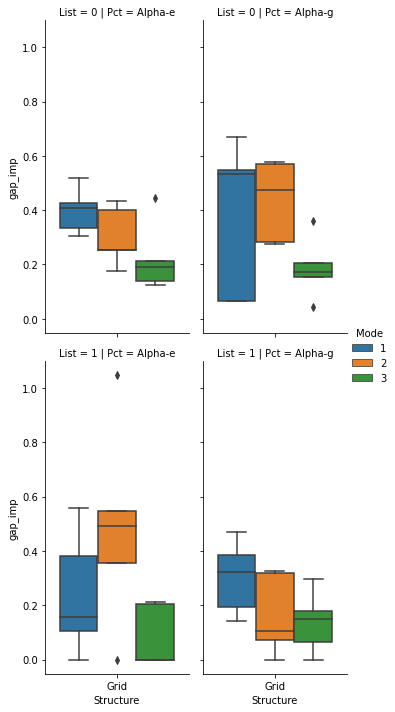
\includegraphics[width=5cm]{improved_gap_ND.png}
\caption{Matheuristic improved gap for \NMD}
\label{fig:4}
\end{figure}
\noindent
The boxplots showed in Figure \ref{fig:4} report the percentage gap of the solution provided by the matheuristic with respect to the one provided by the exact resolution of the MTZ model within the time limit, with initialization by the solution found by the matheuristic.
We can notice that, excluding the outliers, this gap ranges between 0$\%$ and 0.7$\%$ and its lowest values are observed for the instances in which the network where the mothership moves has a star structure (green boxplots). 
From the previous observations, similarly to the \AMD, we can conclude that the behaviour of the matheuristic is very good in terms of quality of the solutions provided, even if the initialization of the MTZ model does not help in speeding up the convergence to the optimal solution. 



\section{Concluding remarks}
\noindent
This papers has analyzed the coordination problem that arises between a mothership vehicle and a drone that must adjust their routes to minimize travel distances while visiting a set of targets modeled by graphs. We have presented exact formulations for different versions of the problem depending on the constraints imposed to the mothership movement (free on a continuous space or on a given network). Our computational results show that the considered problem is rather hard and only small to medium size problems can be  solved to optimality. Additionally, we have proposed a matheuristic algorithm, applicable to all the versions of the problem with minimum changes, that provides acceptable feasible solutions in short computing time;  so that it is a good alternative to the exact methods.\\
\noindent
Further research in this topic includes the coordination of the operations of several drones with a mothership, the possibility of visiting more than one target per operation and combinations of both cases. These problems being very interesting are beyond the scope of this paper and will be the focus of a follow up paper.







